% CS701 final report, Team 7. CVPR two-column template (cvpr.sty from the CVPR 2026 author kit;
% swap in the course's CVPR 2027 cvpr.sty if it differs). Compile: latexmk -pdf main.tex
\documentclass[10pt,twocolumn,letterpaper]{article}

\usepackage{cvpr}              % final (camera-ready) mode: no line numbers
\usepackage{graphicx}
\usepackage{amsmath,amssymb}
\usepackage{booktabs}
\usepackage{multirow}
\usepackage{xcolor}
\usepackage{tikz}
\usetikzlibrary{positioning,arrows.meta,fit,backgrounds,calc}
\definecolor{cvprblue}{rgb}{0.21,0.49,0.74}
\definecolor{navy}{HTML}{141B3D}
\definecolor{tblue}{HTML}{2E4A8B}
\definecolor{amber}{HTML}{F2A900}
\definecolor{amberlt}{HTML}{FDF0C8}
\definecolor{greylt}{HTML}{EEF1F7}
\definecolor{greymd}{HTML}{A3ACC0}
\usepackage[pagebackref,breaklinks,colorlinks,allcolors=cvprblue]{hyperref}

\def\paperID{7}
\def\confName{CVPR}
\def\confYear{2027}

\newcommand{\dm}{\ensuremath{\Delta m}}
\newcommand{\pmm}[1]{\ensuremath{\pm#1}}

\title{One Frozen DINOv3, Wide LoRA and a Tiny-Object Cascade:\\Multi-Task Learning on SAR Images under a 40\,M Budget}

\author{Rayner Sim Zhi Heng\qquad Chen Junkai\qquad Pei Jinling\qquad Le Ba Luat\\
CS701 Deep Learning and Vision, Team 7, Singapore Management University
}

\begin{document}
\maketitle

\begin{abstract}
One model must classify a synthetic aperture radar (SAR) image into nine scene classes and detect all of its objects, half of which are smaller than one $16{\times}16$ ViT patch, with at most 130\,M parameters, 40\,M of them trainable, and one forward pass at $\le512$\,px.
We keep a DINOv3 ViT-B/16 frozen and spend the trainable budget on rank-80 LoRA and a three-stage Cascade R-CNN rebuilt for tiny boxes: 6\,px anchors matched by $\max(\mathrm{IoU},\mathrm{NWD})$, IoU thresholds that relax with box size, a pixel-level CNN prior, and a fix for a $-0.3$\,px annotation bias that ordinary flips double.
Zero-cost steps on one set of weights (checkpoint averaging, image--box score fusion, soft-NMS and snapping to an annotation lattice) add a further ${\approx}3.6$\,\dm.
The entry scores \dm{} 56.49 on the validation board and 61.25 on the test board (macro-F1 96.96, mAP 55.74), third of nine teams at the 8 Nov board snapshot.
A parallel CNN line (YOLO11, ConvNeXt Cascade R-CNN) plateaued at \dm{} 40.35, and three cases show that gains seen in short runs or on one local holdout shrink by $5$--$10\times$ or vanish on the board.
\end{abstract}

%-------------------------------------------------------------------------
\section{Introduction}
\label{sec:intro}

SAR sensors image the ground day and night through cloud, which makes them valuable for monitoring ports, airports and energy infrastructure. A SAR image is a map of microwave backscatter, not a photograph: it is single-channel, covered in multiplicative speckle, and an object often appears as a few bright scatterers next to a dark shadow. Generic vision models are therefore not obviously transferable, and SAR-specific pretraining is excluded by the course rules.

The task couples two outputs from one image: a scene label (macro-F1) and boxes for every object of that class (COCO mAP@[.5:.95]). Teams are ranked by
\begin{equation}
\dm = 50\Big[\tfrac{F1-F1_\text{ref}}{F1_\text{ref}} + \tfrac{\text{mAP}-\text{mAP}_\text{ref}}{\text{mAP}_\text{ref}}\Big],
\end{equation}
with a ViT-B + LoRA reference of 93.31 / 26.13 on validation and 93.99 / 25.41 on test. Since $F1_\text{ref}$ is already high, one mAP point is worth 1.91\,\dm{} and one F1 point only 0.54: \textbf{the score is earned by detection}, which became our first design decision.

Three properties of the data then shaped the model (\cref{fig:data}). (i) \textbf{Boxes are tiny}: 18.4\% of the 32{,}533 boxes have side $<8$\,px and 50.5\% are below 16\,px, \ie below one ViT token. (ii) \textbf{Localisation, not recognition, is the bottleneck}: our AP falls from ${\approx}75$ at IoU\,0.5 to ${\approx}22$ at 0.9. (iii) \textbf{Annotations carry structure}: a systematic sub-pixel offset, an integer coordinate lattice for some classes, about 10\% near-duplicate images, and two classes (bridge, playground) whose labels appear only partly recoverable from SAR.

Our objectives were therefore to (1) adapt a strong generic backbone within 40\,M trainable parameters without destroying its features, (2) make a ViT detector work below its patch size, (3) extract every zero-cost gain from a single forward pass, and (4) build an evaluation protocol that tells real gains from noise. Our contributions are a tiny-object Cascade on a frozen DINOv3, a set of data-driven processing steps, and a candid account of what did not transfer from local runs to the board.

\begin{figure}[t]
  \centering
  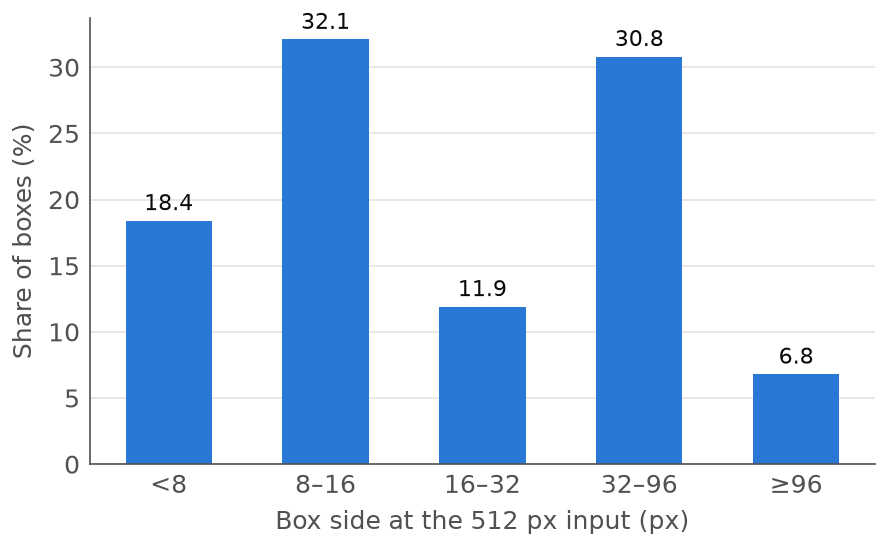
\includegraphics[width=0.49\linewidth]{figures/box_sizes.png}\hfill
  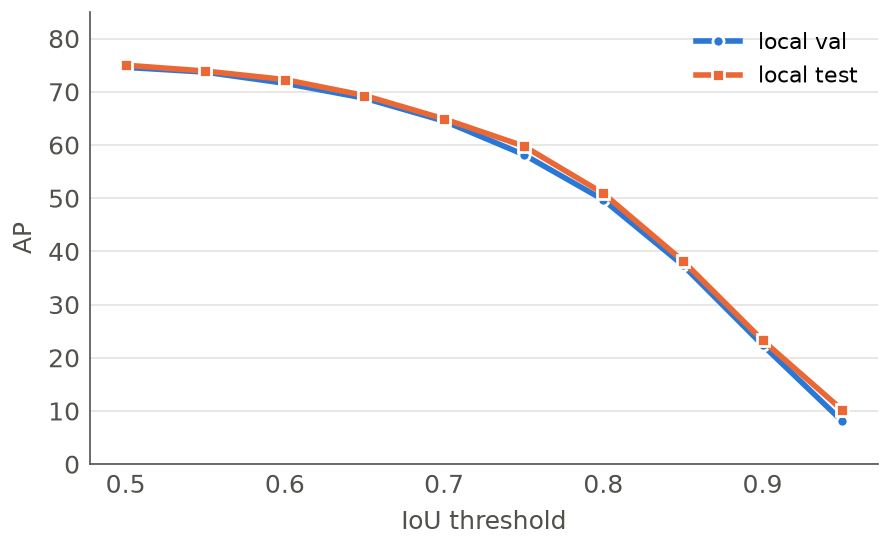
\includegraphics[width=0.49\linewidth]{figures/ap_vs_iou.png}
  \caption{Left: share of boxes by side $\sqrt{wh}$ at the 512\,px input; half are below the 16\,px patch size. Right: AP against IoU threshold on our two local holdouts; the loss concentrates at strict IoU.}
  \label{fig:data}
\end{figure}

%-------------------------------------------------------------------------
\section{Related work}
\label{sec:related}

\textbf{Multi-task learning.} Hard parameter sharing with task heads is the simplest MTL design; loss weighting \cite{kendall2018uncertainty} and task-specific attention \cite{maninis2019mtl} address task interference, and \dm{} is the standard summary metric \cite{vandenhende2021mtl}. Here the two tasks are strongly aligned (every box shares the image class), so interference is small; we found it more useful to let each task inform the other at inference (score fusion, \cref{sec:pp}) than to tune loss weights.

\textbf{Parameter-efficient adaptation.} LoRA \cite{hu2022lora} adds low-rank updates to frozen weights, and MTLoRA \cite{agiza2024mtlora} splits them into shared and task-specific parts. LoRA keeps pretrained features intact and is cheap to store, but its capacity is bounded by the rank; full fine-tuning of a few blocks is the main alternative. We compare both under the same budget (\cref{sec:unfreeze}).

\textbf{Backbones.} Self-supervised ViTs such as DINOv2/v3 \cite{oquab2024dinov2,simeoni2025dinov3} give strong dense features, but a stride-16 token map \cite{dosovitskiy2021vit} has no pixel detail for 8\,px objects. CNNs such as ConvNeXt \cite{liu2022convnext} keep stride-4 features and fit the budget when fully trained, but their supervised ImageNet features transferred worse to SAR in our tests.

\textbf{Detectors.} Two-stage detectors \cite{ren2015faster} with FPN \cite{lin2017fpn} are accurate but tied to anchors; Cascade R-CNN \cite{cai2018cascade} refines boxes in stages with rising IoU thresholds, which directly targets strict-IoU AP. One-stage YOLO detectors \cite{redmon2016yolo} and DETR-style real-time detectors \cite{zhao2024rtdetr} are fast and simple to train, but in our runs they were weaker at strict IoU on tiny boxes. ViTDet \cite{li2022vitdet} builds a pyramid from a single ViT map, and ViT-Adapter \cite{chen2023vitadapter} injects a CNN spatial prior; we use both ideas in reduced form.

\textbf{Tiny objects.} IoU is unstable for small boxes: a 2\,px offset already drives the IoU of an 8\,px box towards zero. NWD \cite{wang2021nwd} models boxes as Gaussians and replaces IoU in assignment. Soft-NMS \cite{bodla2017softnms} keeps overlapping true positives, and weight averaging along a trajectory \cite{izmailov2018swa,wortsman2022soups} improves a single model at no inference cost.

%-------------------------------------------------------------------------
\section{Method}
\label{sec:method}

\begin{figure*}[t]
\centering
\resizebox{\textwidth}{!}{%
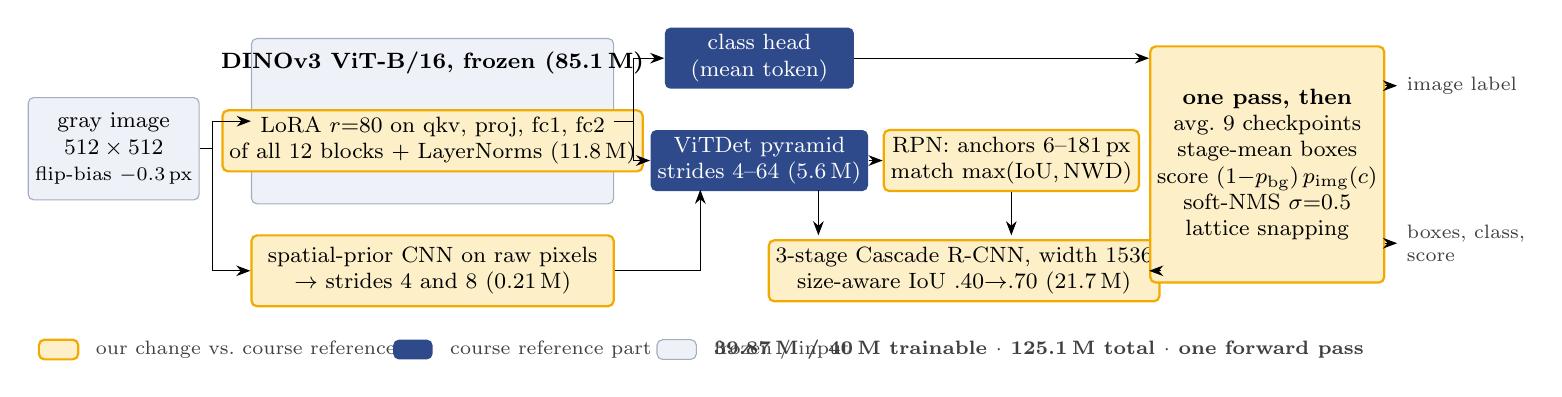
\begin{tikzpicture}[
  font=\footnotesize, >={Stealth[length=1.8mm]}, x=1cm, y=1cm,
  blk/.style={rounded corners=2pt, align=center, inner sep=2.5pt},
  ours/.style={blk, fill=amberlt, draw=amber, line width=0.8pt},
  ref/.style={blk, fill=tblue, text=white},
  frz/.style={blk, fill=greylt, draw=greymd},
  lab/.style={font=\scriptsize, text=black!75, align=left}]
  \node[frz, minimum width=1.9cm, minimum height=1.3cm] (in) at (0.95,0.1) {gray image\\$512\times512$\\{\scriptsize flip-bias $-0.3$\,px}};
  \node[frz, minimum width=4.6cm, minimum height=2.1cm] (vit) at (5.0,0.45) {};
  \node[font=\footnotesize\bfseries, anchor=north] at (5.0,1.45) {DINOv3 ViT-B/16, frozen (85.1\,M)};
  \node[ours, minimum width=4.2cm] (lora) at (5.0,0.2) {LoRA $r{=}80$ on qkv, proj, fc1, fc2\\of all 12 blocks + LayerNorms (11.8\,M)};
  \node[ours, minimum width=4.6cm, minimum height=0.9cm] (prior) at (5.0,-1.45) {spatial-prior CNN on raw pixels\\$\to$ strides 4 and 8 (0.21\,M)};
  \node[ref, minimum width=2.4cm] (cls) at (9.15,1.25) {class head\\(mean token)};
  \node[ref, minimum width=2.4cm] (fpn) at (9.15,-0.05) {ViTDet pyramid\\strides 4--64 (5.6\,M)};
  \node[ours, minimum width=3.0cm] (rpn) at (12.35,-0.05) {RPN: anchors 6--181\,px\\match $\max(\mathrm{IoU},\mathrm{NWD})$};
  \node[ours, minimum width=4.4cm] (cas) at (11.75,-1.45) {3-stage Cascade R-CNN, width 1536\\size-aware IoU .40$\to$.70 (21.7\,M)};
  \node[ours, minimum width=2.7cm, minimum height=3.0cm] (pp) at (15.6,-0.1) {\textbf{one pass, then}\\avg.\ 9 checkpoints\\stage-mean boxes\\score $(1{-}p_\text{bg})\,p_\text{img}(c)$\\soft-NMS $\sigma{=}0.5$\\lattice snapping};
  \node[lab, anchor=west] (o1) at (17.25,0.9) {image label};
  \node[lab, anchor=west] (o2) at (17.25,-1.1) {boxes, class,\\score};
  \draw[->] (in.east) -- (2.2,0.1) |- (vit.west);
  \draw[->] (2.2,0.1) |- (prior.west);
  \draw[->] (vit.east) -- (7.55,0.45) |- (cls.west);
  \draw[->] (7.55,0.45) |- (fpn.west);
  \draw[->] (prior.east) -- (8.4,-1.45) -- (8.4,-0.42);
  \draw[->] (fpn) -- (rpn);
  \draw[->] (rpn.south) -- (12.35,-1.0);
  \draw[->] (9.9,-0.42) -- (9.9,-1.0);
  \draw[->] (cas.east) -- (pp.west |- cas.east);
  \draw[->] (cls.east) -- (pp.west |- cls.east);
  \draw[->] (pp.east |- o1.west) -- (o1.west);
  \draw[->] (pp.east |- o2.west) -- (o2.west);
  \node[ours, minimum height=0.25cm, minimum width=0.5cm, inner sep=0pt] (l1) at (0.25,-2.45) {};
  \node[lab, anchor=west] (t1) at (0.6,-2.45) {our change vs.\ course reference};
  \node[ref, minimum height=0.25cm, minimum width=0.5cm, inner sep=0pt] (l2) at (4.75,-2.45) {};
  \node[lab, anchor=west] (t2) at (5.1,-2.45) {course reference part};
  \node[frz, minimum height=0.25cm, minimum width=0.5cm, inner sep=0pt] (l3) at (8.1,-2.45) {};
  \node[lab, anchor=west] at (8.45,-2.45) {frozen / input};
  \node[lab, anchor=east, font=\scriptsize\bfseries] at (16.95,-2.45) {39.87\,M / 40\,M trainable $\cdot$ 125.1\,M total $\cdot$ one forward pass};
\end{tikzpicture}}
\caption{Final model. Amber blocks are our changes to the course reference (ViT-B + LoRA + Faster R-CNN). Each image goes through the network once; everything in the right-hand box uses only that forward pass.}
\label{fig:pipeline}
\end{figure*}

\Cref{fig:pipeline} shows the final model; each part below states what we changed and why.

\textbf{Backbone and adaptation.} We use timm's DINOv3 ViT-B/16 (LVD-1689M) and sum the RGB patch kernel into one gray channel, so the pretrained weights are reused exactly on SAR input. The backbone stays frozen. LoRA of rank 80 ($\alpha{=}160$) is added to qkv, proj, fc1 and fc2 in all 12 blocks, and the LayerNorms train. Images of 256 or 224\,px are stretched to 512, which the rules allow (one pass, at most $512^2$, no tiling).

\textbf{Pyramid and spatial prior.} A ViTDet-style pyramid (strides 4--64, 256 channels) is built from the last token map. Because a stride-16 map has no detail for sub-patch objects, a randomly initialised 64-channel CNN (0.21\,M parameters) reads the raw image and is added to the stride-4 and stride-8 levels through zero-initialised $1{\times}1$ convolutions, so training starts from the unmodified pyramid.

\textbf{Tiny-object RPN.} Anchors range over 6--181\,px and sit at cell centres. Positives are assigned by $\max(\mathrm{IoU},\mathrm{NWD})$ with $C{=}8$, so 8\,px objects that IoU would reject still receive anchors.

\textbf{Size-aware Cascade.} The standard 0.5/0.6/0.7 stage thresholds leave tiny objects without positives in later stages. We use thresholds that depend on GT side: .40/.45/.50 below 8\,px, .45/.50/.55 for 8--16\,px, .50/.55/.65 for 16--32\,px, and .5/.6/.7 above. Heads are class-agnostic, 1536 wide, with aligned RoIAlign.

\textbf{Flip-bias correction.} Boxes carry a systematic offset of about $-0.3$\,px. A horizontal flip mirrors it, so flipped targets disagree with unflipped ones by twice the bias; our flip moves flipped boxes back by $-0.3$\,px.

\textbf{Training.} Flips only (rotations hurt; see \cref{sec:failed}); AdamW, LR $10^{-4}$ for heads and $3{\times}10^{-4}$ for LoRA, weight decay 0.05, batch 16, a 200-epoch cosine schedule, and all 9{,}392 labelled images for the submitted model. Training took 13\,h on two RTX 6000 Ada GPUs.

\subsection{Single-pass post-processing}
\label{sec:pp}
\textbf{Checkpoint averaging.} The weights at epochs 100, 110, \dots, 180 of one run are averaged into one model, which still costs one forward pass. \textbf{Box score.} With $p$ the stage-averaged box class probabilities and $p_\text{img}$ the image classifier, $s_c=(1-p_\text{bg})\,p_\text{img}(c)$, without RPN objectness. This class-agnostic fusion lets the image prior suppress other-class false positives without deleting boxes in misclassified images. \textbf{Boxes} are the mean of the three stages, shifted by $-0.2$\,px, with per-class Gaussian soft-NMS ($\sigma{=}0.5$), and at least 100 boxes are kept per image. \textbf{Image label} is $\arg\max_c[\log p_\text{img}(c)+2\log\max_i p_i(c)]$, so confident detections can correct the classifier. \textbf{Lattice snapping.} All training boxes of aircraft, car and every 256\,px image have integer coordinates in original pixels, and about 40\% of wind-turbine images share one fractional offset. We round predicted corners onto that lattice; for wind turbines a per-image circular-mean offset is applied when its concentration $R\ge0.5$. Scores and ranking are unchanged.

\subsection{A parallel CNN detector line}
\label{sec:cnn}
To test whether a convolutional design with native stride-4 features suits 8\,px targets better, one of us developed a CNN line on the same split and protocol. It started from YOLO11-L (COCO-pretrained) and moved to a torchvision Faster/Cascade R-CNN on a ConvNeXt-T/S backbone (ImageNet-22k) with an FPN over P2--P6. The ConvNeXt-S version keeps the stem and early stages trainable and freezes part of stage 2, giving 62.6\,M total and 39.5\,M trainable parameters. RPN and RoI computations had to stay in FP32, because bf16 autocast snapped boxes to a 2\,px grid. The line then added the same kinds of change as the main model: soft-NMS, image--box score fusion, the box shift, and later 6\,px anchors, an NWD term in the RPN and size-aware IoU.

\subsection{Spending the budget on full blocks}
\label{sec:unfreeze}
LoRA of rank 80 everywhere is one way to spend 40\,M parameters. The alternative trains the \emph{last two ViT blocks fully} (14.2\,M), uses LoRA of rank 48 on the other ten blocks and a 1024-wide head (39.15\,M trainable). We screened this and two spatial-prior variants on the team code, then trained the winner at full length.

%-------------------------------------------------------------------------
\section{Experiments and analysis}
\label{sec:exp}

\textbf{Protocol.} Screens use a class-stratified split of the training set (7{,}512 / 940 / 940). Ablations for this report use a second split, \emph{vallike}: 992 held-out images sampled to match the predicted class and image-size mix of the official validation set, with the other 8{,}400 images for training. Official validation and test images were only ever predicted. Repeating one 36-epoch configuration with 37 seeds gave a standard deviation of $\pm0.70$ local \dm, so differences between single runs below ${\approx}1$\,\dm{} are noise. Post-processing comparisons are paired on the same weights, so 0.1--0.3\,\dm{} differences can be real there.

\subsection{Main result and progression}

\begin{table}[t]
\centering\small
\setlength{\tabcolsep}{2.4pt}
\begin{tabular}{@{}llccc@{}}
\toprule
Entry & Main change & F1 & mAP & \dm \\
\midrule
V2  & DINOv3 + LoRA + Cascade, 120 ep & 95.06 & 45.62 & 38.23 \\
F2  & + size-aware IoU, flip bias, all data & 95.46 & 48.97 & 44.84 \\
SC2 & LoRA r80, head 1536, 150 ep & 95.35 & 52.66 & 51.86 \\
BP7 & + spatial prior, cosine 160 & 95.35 & 53.15 & 52.78 \\
cos200 & cosine 200, e160 & 95.02 & 53.56 & 53.41 \\
 & + post-proc.\ (\cref{sec:pp}) & 95.09 & 54.29 & 54.83 \\
 & + avg.\ 9 ckpts, agn.\ fusion & 95.27 & 55.10 & \textbf{56.49} \\
\midrule
\multicolumn{2}{@{}l}{Test entry (intended recipe + snapping)} & 96.96 & 55.74 & \textbf{61.25} \\
\bottomrule
\end{tabular}
\caption{Official scores (validation board; last row test board, with its own reference). Steps change several things at once; \cref{tab:loo,tab:pp} attribute them.}
\label{tab:official}
\end{table}

\Cref{tab:official} traces the official score. The largest single jump (F2$\to$SC2, $+7.0$\,\dm) came from filling the budget with a wider LoRA and head together with a longer schedule; slower cosines helped twice ($+1.3$, $+0.6$), and the last $3.1$\,\dm{} on validation needed no training at all. We finished Phase 1 third of nine and were third of nine on the test board at the 8 Nov snapshot (the board closed later that day). Our test macro-F1 (96.96) is above both leading teams (96.11, 96.27), whereas their mAP is 5.5 points higher (61.2 \vs 55.7) while their AP50 is only 2.6 higher, so the remaining gap is at strict IoU.

\subsection{What each part adds}

\begin{table}[t]
\centering\small
\setlength{\tabcolsep}{2.4pt}
\begin{tabular}{@{}lccc@{}}
\toprule
Variant (one part removed) & Train.\,M & mAP & $\Delta\dm$ \\
\midrule
Final recipe & 39.87 & 45.76\pmm{0.09} & -- \\
no Cascade (Faster R-CNN) & 32.16 & 42.23\pmm{0.34} & $-7.09$\pmm{0.46} \\
LoRA r32, head 1024 & 24.02 & 43.87\pmm{0.35} & $-3.63$\pmm{0.49} \\
no size-aware IoU & 39.87 & 44.60\pmm{0.53} & $-2.31$\pmm{1.11} \\
reference anchors & 39.86 & 44.87\pmm{0.33} & $-1.86$\pmm{0.80} \\
no flip-bias fix & 39.87 & 44.88\pmm{0.43} & $-1.54$\pmm{0.84} \\
no spatial prior & 39.66 & 45.47\pmm{0.35} & $-0.71$\pmm{0.40} \\
LayerNorms frozen & 39.83 & 45.75\pmm{0.15} & $-0.13$\pmm{0.29} \\
no NWD matching & 39.87 & 46.10\pmm{0.51} & $+0.60$\pmm{1.20} \\
\bottomrule
\end{tabular}
\caption{Leave-one-out on \emph{vallike} (36-epoch cosine, full post-processing; mean\,$\pm$\,std over 3 seeds, paired by seed). Short runs rank parts but understate parts that pay late.}
\label{tab:loo}
\end{table}

\begin{table}[t]
\centering\small
\begin{tabular}{@{}lcc@{}}
\toprule
Step (cumulative, fixed weights) & $\Delta$mAP & $\Delta\dm$ \\
\midrule
soft-NMS $\sigma$ 0.75$\to$0.5 & $+0.16$ & $+0.30$\pmm{0.02} \\
drop RPN objectness & $+0.39$ & $+0.75$\pmm{0.25} \\
RPN top 2000, image-label $\lambda{=}2$ & $+0.03$ & $+0.14$ \\
average checkpoints e100--180 & $+0.73$ & $+1.38$\pmm{0.17} \\
image--box score fusion (class-agn.) & $+0.22$ & $+0.41$ \\
min-keep 100 & $+0.02$ & $+0.04$ \\
lattice snapping & $+0.32$ & $+0.62$\pmm{0.21} \\
\midrule
total & $+1.87$ & $\approx\!+3.6$ \\
\bottomrule
\end{tabular}
\caption{Zero-training steps on full-length runs (\emph{vallike}, 3 seeds; final mAP 58.74\pmm{0.09}).}
\label{tab:pp}
\end{table}

\Cref{tab:loo} removes one part at a time. The cascade is the most valuable part ($-7.1$\,\dm{} without it), confirming that the bottleneck is box quality. Capacity is next: shrinking LoRA and the head to 24\,M costs 3.6\,\dm. All three tiny-object changes help (size-aware IoU, small anchors, flip bias, together ${\approx}5.7$\,\dm). NWD matching shows no stable benefit once the other tiny-object parts are present: seed 0 declines and seeds 1--2 improve. Earlier single-seed screens on the 7{,}512 split ranked the same parts in the same order: DINOv3 instead of ImageNet-21k ViT gave $+8.1$ local \dm, LoRA on all linear layers $+18.1$, and the cascade $+21.0$.
\Cref{tab:pp} shows the zero-training steps. Checkpoint averaging is the largest ($+1.38$\,\dm). The flat, low-LR tail of the 200-epoch cosine is exactly where averaging helps. Dropping RPN objectness from the score helps because objectness is poorly calibrated for tiny boxes. Snapping is the only data-mining finding that survived testing: $+0.20$ and $+0.36$ mAP on two holdouts (paired bootstrap $P{\approx}1$).

\subsection{The CNN line and full-block adaptation}

\begin{figure*}[t]
  \centering
  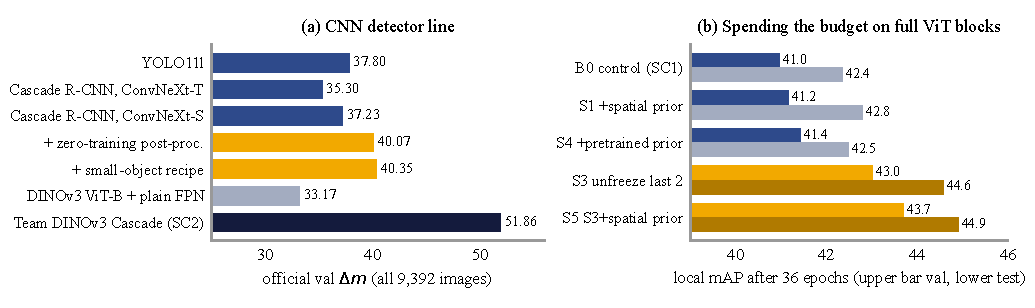
\includegraphics[width=\linewidth]{figures/cnn_and_unfreeze.pdf}
  \caption{(a) Official validation \dm{} of the CNN detector line, all trained on the full training set; amber steps reuse the main model's ideas. (b) Screens on the team code at 36 epochs: training the last two ViT blocks fully (amber) leads by ${\approx}2$ mAP on both local splits, but the lead shrinks to $+0.25$ mAP at 150 epochs on the board (\cref{sec:lessons}).}
  \label{fig:cnn}
\end{figure*}

\textbf{CNN line} (\cref{fig:cnn}a). YOLO11-L trained on all data reached 37.8 on the board. Faster R-CNN on ConvNeXt-T gave the best macro-F1 of any model at that time (95.3 local) but loose boxes: AP50 was 5 points and AP75 15 points below YOLO11-L. This led to a three-stage cascade and the larger ConvNeXt-S (35.3$\to$37.2). The zero-training steps transferred directly: soft-NMS, score fusion and the box shift gave $+2.8$\,\dm{} on the board with the same weights (mAP 45.0$\to$46.4). The small-object recipe then added only $+0.3$ (46.5 mAP). DETR-style detectors trailed YOLO11-L on our split (DEIMv2-L $-3.4$\,mAP at 48 epochs, RF-DETR-S ${\approx}-12$), and DINOv3 ViT-B with LoRA behind a plain FPN in the same R-CNN scored only 33.2. The main model differs in its ViTDet neck with normalised per-level convolutions, final-norm tokens and a wider cascade head; we did not isolate which of these mattered. With the main line 11\,\dm{} ahead, we moved this compute to it.

\textbf{Full blocks \vs wide LoRA} (\cref{fig:cnn}b). At 36 epochs, training the last two blocks fully (S3) beat the control by $+2.06$ / $+2.21$ mAP on the two local splits, with gains on harbor, wind turbine and airport. Pretrained or random spatial priors added at most $0.4$. A doubled LR diverged. Trained for 150 epochs on all data, however, S3 scored 52.91 mAP on the validation board against 52.66 for the same-length SC2 (+0.25), and averaging epochs 120--140 reached mAP 53.03 / \dm{} 52.56. That is still below BP7, so the final model kept rank-80 LoRA.

\subsection{Data findings and the weak classes}
\label{sec:weak}

\begin{figure}[t]
  \centering
  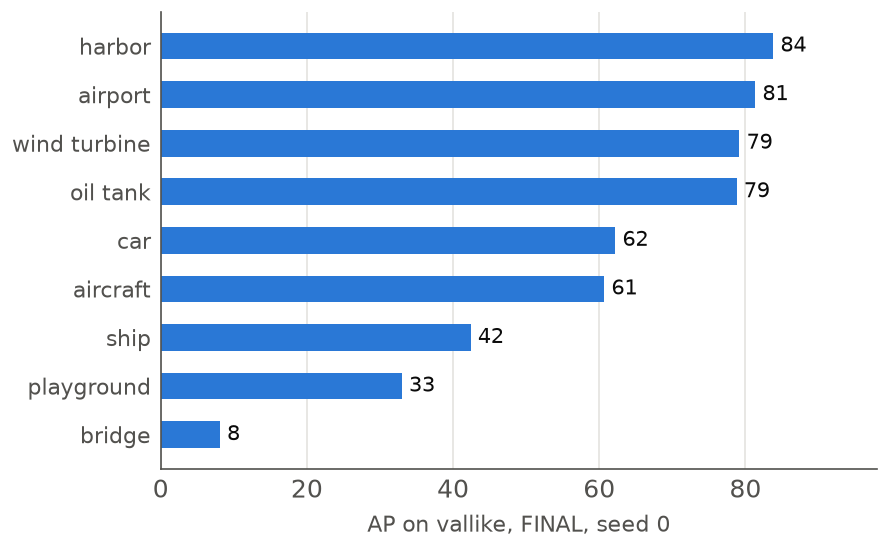
\includegraphics[width=0.49\linewidth]{figures/per_class_ap.png}\hfill
  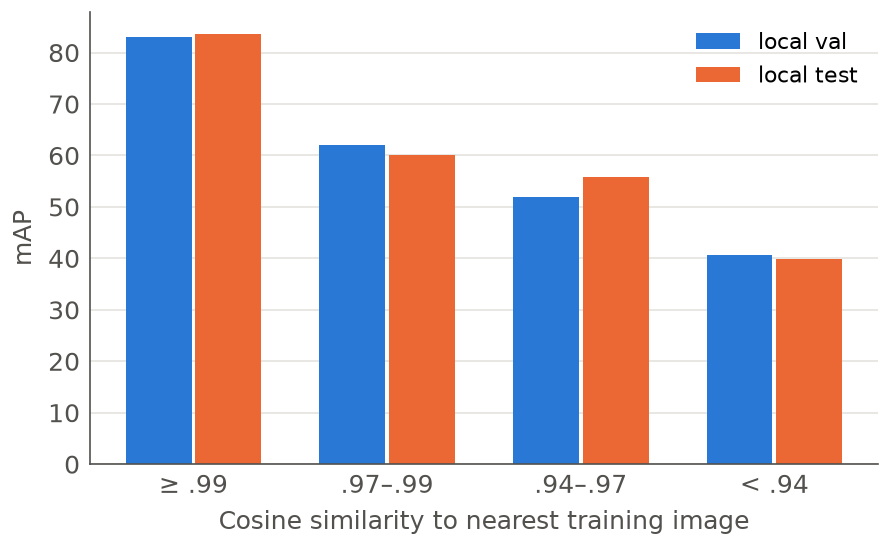
\includegraphics[width=0.49\linewidth]{figures/near_duplicates.png}
  \caption{Left: per-class AP of the final recipe on \emph{vallike}. Right: mAP by similarity to the nearest training image (frozen DINOv3 cosine).}
  \label{fig:weak}
\end{figure}

\begin{figure}[t]
  \centering
  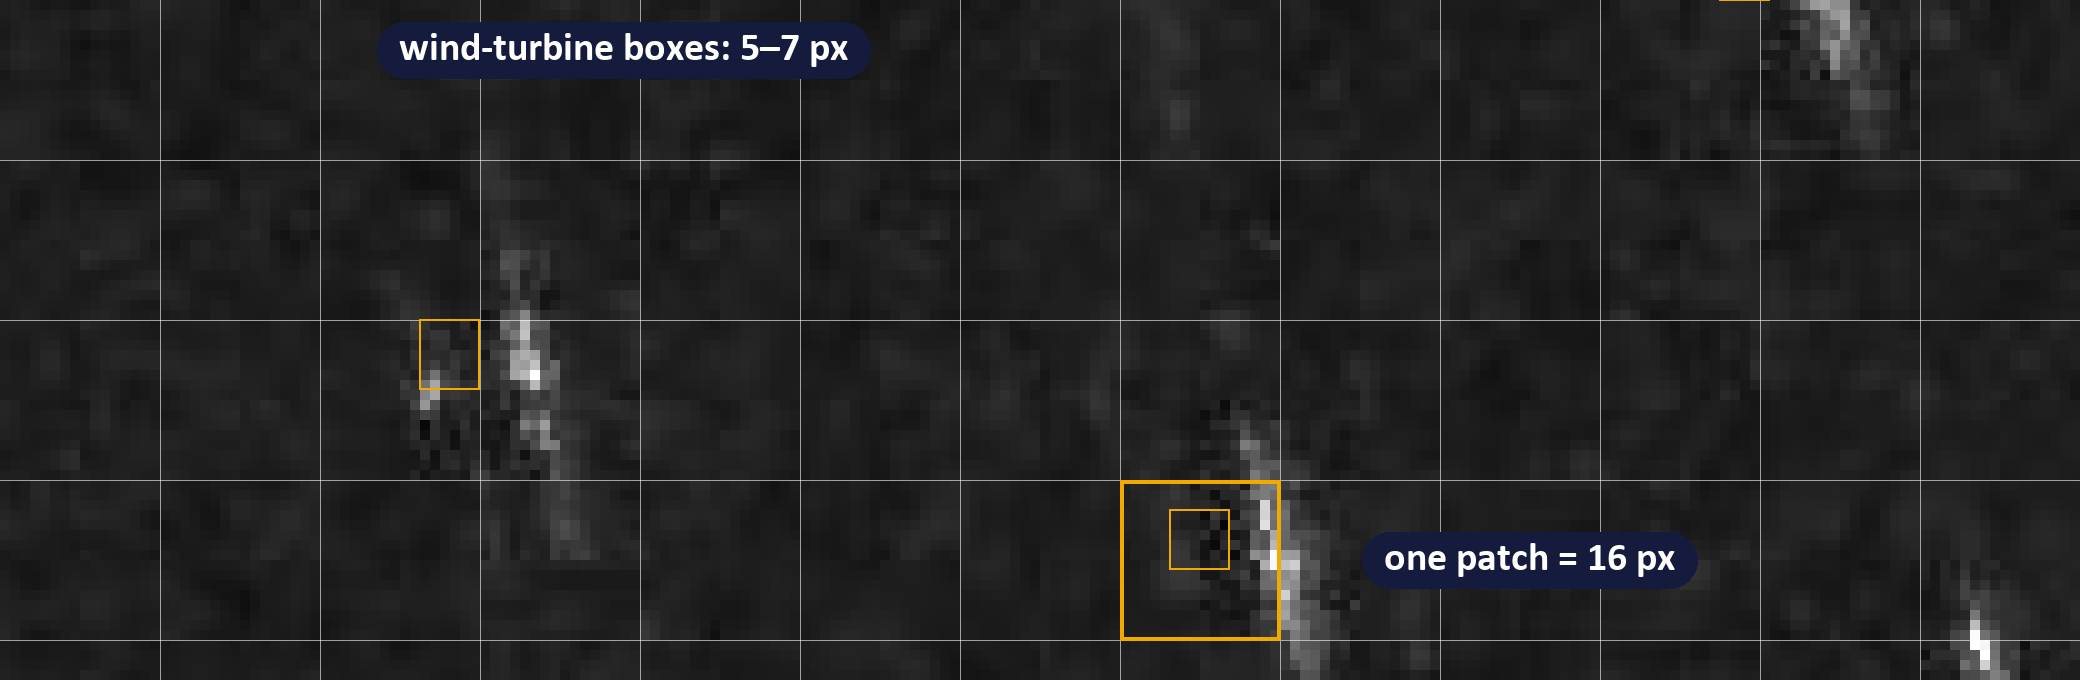
\includegraphics[width=\linewidth]{figures/patchgrid.png}\\[2pt]
  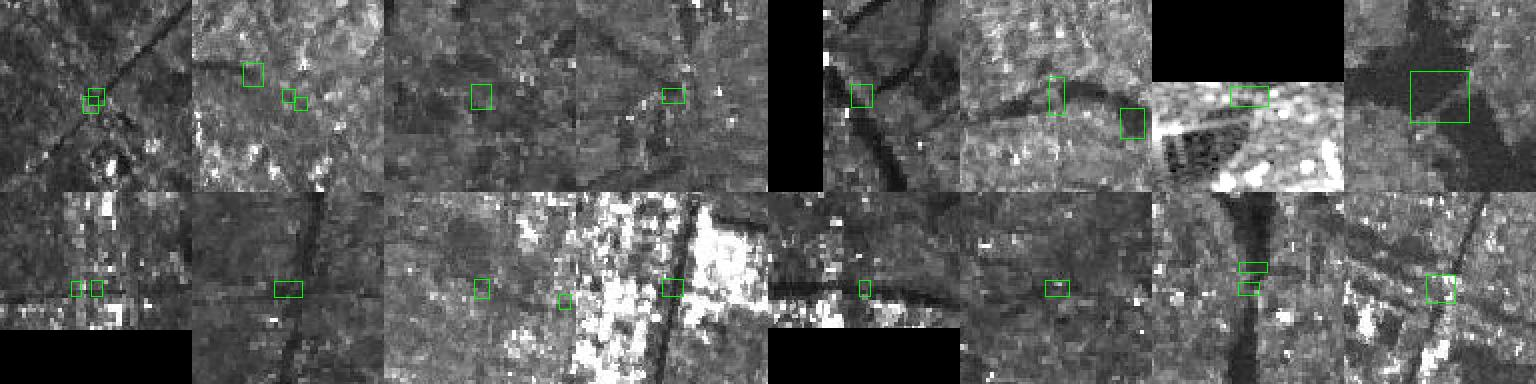
\includegraphics[width=\linewidth]{figures/bridge_gt.png}
  \caption{Visual examples (training images, ground truth). Top: wind turbines; the 5--7\,px boxes sit beside the bright return and inside one 16\,px ViT patch (grid). Bottom: bridge boxes (green), often on dark road crossings with no bright SAR return, which helps explain why bridge AP stays at 8.}
  \label{fig:examples}
\end{figure}

\textbf{Near-duplicates.} About 10\% of holdout images have a near-copy in the training set (\cref{fig:weak}, right). Local mAP is 83 on these against 40 for images without one, and playground AP is 87 against 12. This inflates local scores and is why we built \emph{vallike} and required a second confirmation.

\textbf{Bridge and playground.} Bridge stays at AP 8 and playground at 33 (\cref{fig:weak}, left), although wind turbines, which are smaller, reach 79; size alone is not the cause. Only 53\% / 67\% of their boxes receive a proposal at IoU 0.5 (96\% for wind turbines), and bridge$\leftrightarrow$playground accounts for 24 of 48 image-classification errors. Evidence from the CNN line points to the labels. A YOLO11-L reaches playground AP50 62.5 on its own training images but 6.4 held out, so it memorises rather than generalises. 33\% of bridge and 23\% of playground boxes contain no bright SAR return (7\% for wind turbines, 0\% for ships). Shifting, rescaling or swapping the ground-truth boxes never improved the match (identity was always best), and no image feature separated labelled objects from confident unlabelled detections. Positive-unlabelled loss reweighting (41.28 \vs 41.31 mAP), class weights and oversampling all failed to move bridge by more than 0.9 AP; oversampling also cost $-4.2$\,\dm{} on other classes. We conclude that these labels are only partly recoverable from SAR. This remains a limit of the data, not one we could train away.

\subsection{What did not work}
\label{sec:failed}
\textbf{Augmentation.} $90^\circ$ rotations cost 5--6\,\dm{} on YOLO models and lost 3.7 mAP over 100 epochs on the cascade; copy-paste and zoom also trailed plain flips. We attribute this to SAR geometry: shadow and layover follow the radar look direction, so rotated images are physically implausible. Oversampling images with small objects helped every short run ($+4$ to $+11$\,\dm{} at 24 epochs), but was not tested at full length.
\textbf{Other.} EMA, an IoU branch, a 1024-RoI batch, overlapping patches (stride 8, $2.6\times$ compute), halving the LR ($-7.2$), a LingBot-B backbone, box voting, rank or size priors, and RoI context were all neutral or harmful. RoI context is the most instructive case: $+2.26$\,\dm{} on one holdout, $-0.12$ on the other and $-0.03$ on the board.

\subsection{Lessons on evaluation}
\label{sec:lessons}
Three independent cases show local gains shrinking by $5$--$10\times$ or vanishing on the board. RoI context went from $+2.26$\,\dm{} to $-0.03$. The CNN small-object recipe went from $+1.47$ holdout mAP to $+0.17$ mAP on the board. Full-block adaptation went from $+2.1$ mAP at 36 epochs to $+0.25$ at 150. The causes are near-duplicates, single-holdout variance and parts whose advantage disappears as the LR decays. Our rule became: short runs rank ideas, and a change is kept only when a second holdout, a full-length run or the board agrees.

%-------------------------------------------------------------------------
\section{Conclusion}
A frozen generic backbone (DINOv3), adapted with wide LoRA and paired with a detector rebuilt for sub-patch objects, carried most of the gain, and patient schedules and careful use of one forward pass supplied the rest. The metric decided where effort went: one mAP point is worth 3.6 F1 points. The remaining gap to the leaders, about 5 mAP, lies at strict IoU on tiny boxes and in two classes whose labels SAR does not fully support.
\textbf{Limitations.} The submitted model is a single seed; the ablations are 36-epoch runs, and their absolute \dm{} uses the official reference on a local split. Several Phase 1 choices were made on the validation board, so our validation score is optimistic. Most code was written with AI coding assistants directed by the team.

\textbf{Compliance.} 125{,}076{,}960 total / 39{,}867{,}360 trainable parameters; one gray $512^2$ input, one pass, no TTA or ensembles; pretrained weights DINOv3 LVD-1689M (none trained on SAR); about 514 GPU-hours for the whole project, including tuning.

{
    \small
    \bibliographystyle{ieeenat_fullname}
    \bibliography{main}
}

\end{document}
